% vim:ft=tex:
%
\documentclass[UTF8]{ctexart}
\usepackage{amsmath}
\usepackage{listings}
\usepackage{graphicx}
\usepackage{float}
\usepackage{caption}

\lstset{
    basicstyle          =   \sffamily,          % 基本代码风格
    keywordstyle        =   \bfseries,          % 关键字风格
    commentstyle        =   \rmfamily\itshape,  % 注释的风格,斜体
    stringstyle         =   \ttfamily,  % 字符串风格
    flexiblecolumns,                % 别问为什么,加上这个
    numbers             =   left,   % 行号的位置在左边
    showspaces          =   false,  % 是否显示空格,显示了有点乱,所以不现实了
    numberstyle         =   \zihao{-5}\ttfamily,    % 行号的样式,小五号,tt等宽字体
    showstringspaces    =   false,
    captionpos          =   t,      % 这段代码的名字所呈现的位置,t指的是top上面
    frame               =   lrtb,   % 显示边框
}

\lstdefinestyle{Python}{
    language        =   Python, % 语言选Python
    basicstyle      =   \zihao{-5}\ttfamily,
    numberstyle     =   \zihao{-5}\ttfamily,
    keywordstyle    =   \color{blue},
    keywordstyle    =   [2] \color{teal},
    stringstyle     =   \color{magenta},
    commentstyle    =   \color{red}\ttfamily,
    breaklines      =   true,   % 自动换行,建议不要写太长的行
    columns         =   fixed,  % 如果不加这一句,字间距就不固定,很丑,必须加
    basewidth       =   0.5em,
}
\title{
	第二次作业实验报告
}
\author{
	林乐天 2300012154--- \texttt{yingziyu-Lin@outlook.com}
}

\begin{document}
\maketitle
本次作业分为两个部分,我将从两个部分分别做出实验报告。

\section{numpy for mnist}
\subsection{简述}
这部分作业是让我们用numpy写一个简单的多层感知器,需要实现梯度下降、反向传播等功能。

首先需要定义激活层函数和导数,loss function和其导数。

在本作业中,我使用RELu和softmax作为激活函数,用交叉熵作为loss function

\subsection{流程}
我先做出了一个最基本的模型,一个隐藏层,结果如下:
\begin{figure}[H]
\centering
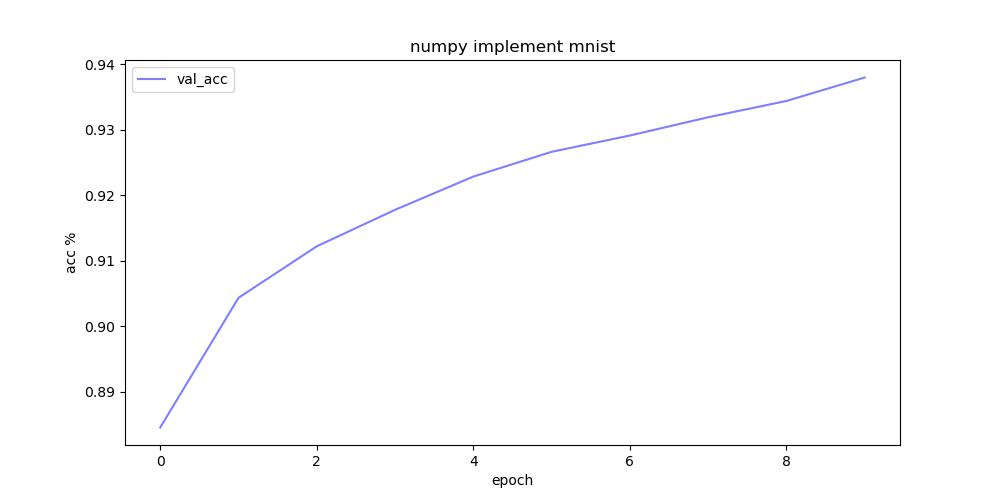
\includegraphics[scale=0.5]{numpy_acc.jpg}
\caption{lr = 0.01}
\end{figure}

发现最后还是没有学习完全,于是我调整了学习率,将学习率增加了5倍。
\begin{figure}[H]
\centering
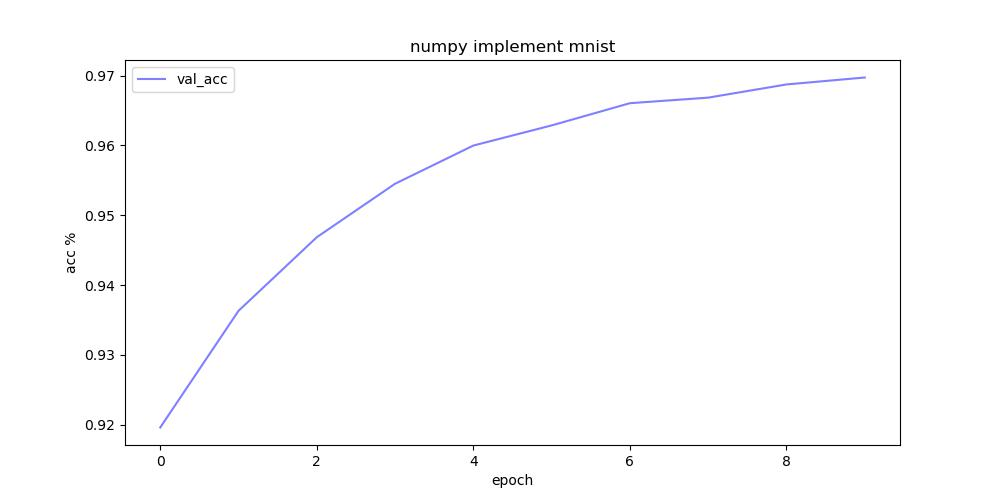
\includegraphics[scale=0.5]{numpy_acc_2.jpg}
\caption{lr = 0.05}
\end{figure}

\section{pytorch}
首先是加了两个隐藏层,将一个的激活函数改成了sigmoid。发现sigmoid在该任务上的效果不好。
\begin{figure}[H]
\centering
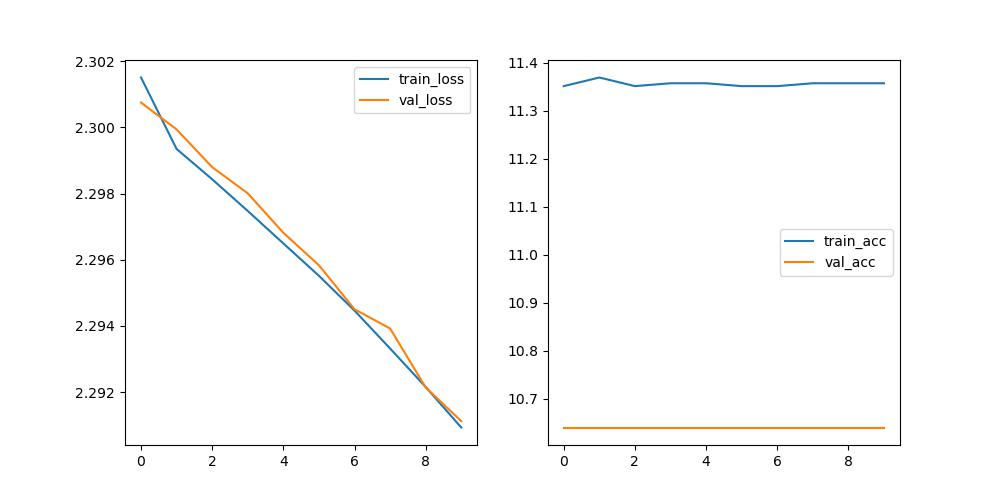
\includegraphics[scale=0.5]{no_dropout_SDG.jpg}
\caption{没有droupout,SDG}
\end{figure}
将优化器换成Adam
\begin{figure}[H]
\centering
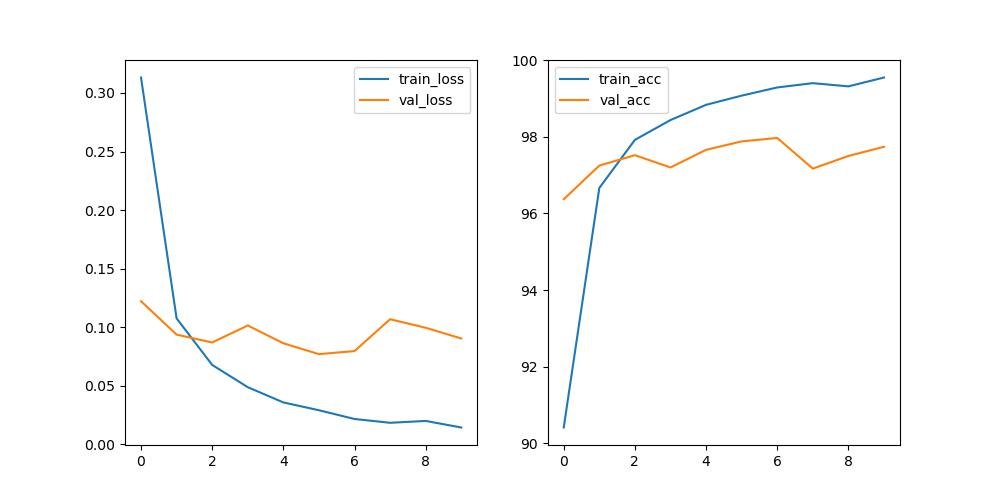
\includegraphics[scale=0.5]{no_dropout.jpg}
\end{figure}

再换成Adadelta
\begin{figure}[H]
\centering
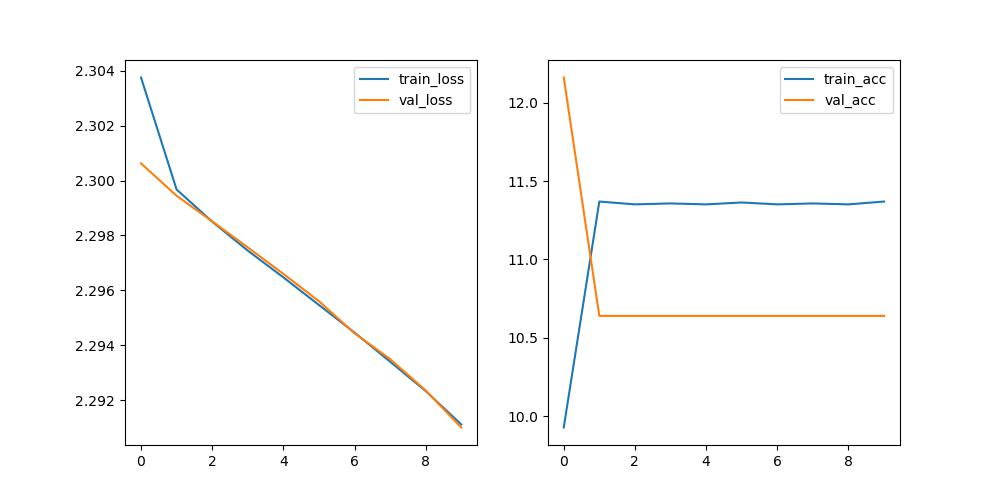
\includegraphics[scale=0.5]{no_dropout_Adadelta.jpg}
\end{figure}

Adam效果最好。

可以看出来,有比较严重的过拟合的情况。加入Dropout层。
\begin{figure}[H]
\centering
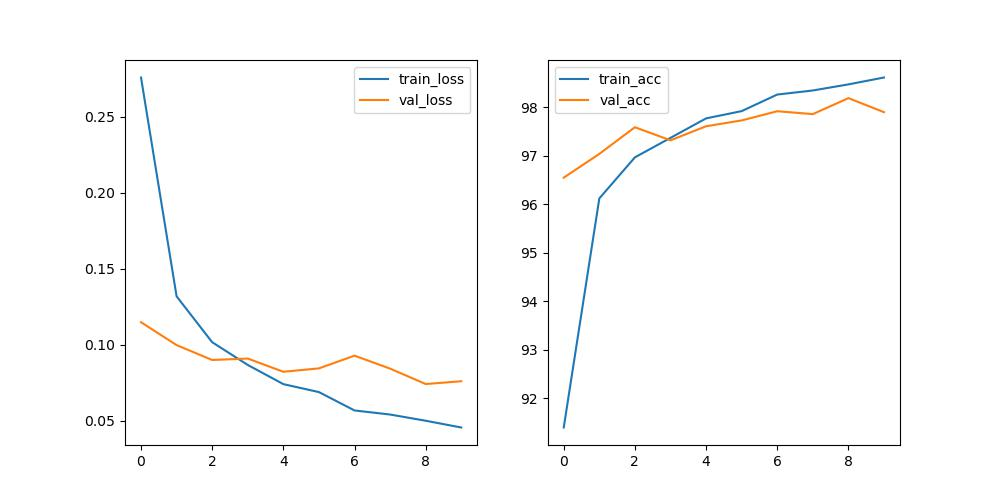
\includegraphics[scale=0.5]{with_dropout.jpg}
\end{figure}

缩小学习率试试
\begin{figure}[H]
\centering
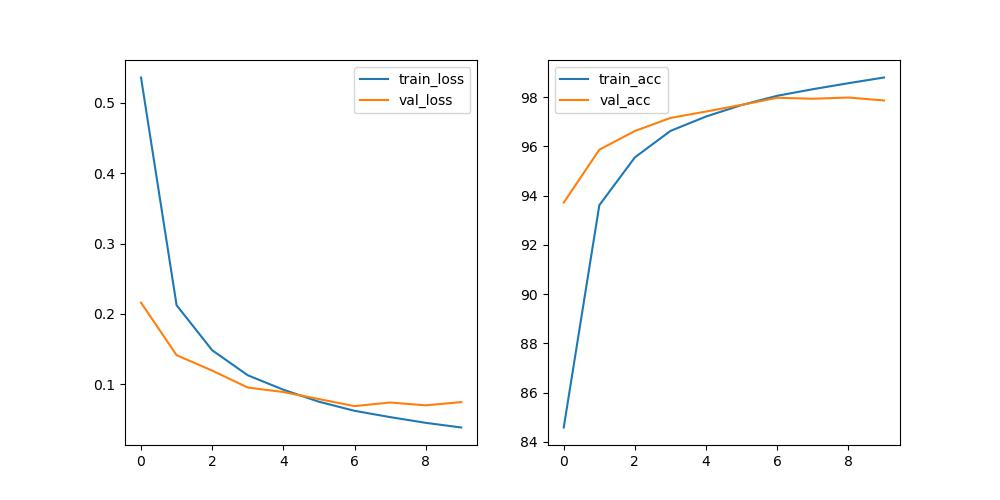
\includegraphics[scale=0.5]{with_dropout_smaller_lr.jpg}
\end{figure}

\end{document}
